\documentclass[11pt,a4paper]{article}
\usepackage[utf8]{inputenc}
\usepackage[unicode]{hyperref}
\usepackage{amsmath}
\usepackage{amssymb}
\usepackage{amsfonts}
\usepackage{geometry}
\usepackage{booktabs}
\usepackage{graphicx}
\usepackage{titlesec}
\usepackage{xcolor} 
\usepackage{fancyhdr}  % For professional headers and footers
\usepackage{parskip}   % For clean block-paragraph spacing
\usepackage{microtype} % Improves overall text justification and hyphenation
\usepackage{float}

%Page Geometry Adjustment
\geometry{top=1.2in, bottom=1.2in, left=1in, right=1in}

%Color Definitions
\definecolor{DeepNavy}{HTML}{1A365D}   % Primary color for main titles/sections
\definecolor{SlateGrey}{HTML}{4A5568}  % Secondary color for text/subtitles
\definecolor{LightIce}{HTML}{F7FAFC}   % Tint color for table rows
\definecolor{MutedBlue}{HTML}{2B6CB0}  % Accent color for subsections

\hypersetup{
    colorlinks=true,
    linkcolor=DeepNavy,
    citecolor=DeepNavy,
    urlcolor=MutedBlue,
    pdfborder={0 0 0}
}

%Header and Footer Configuration
\pagestyle{fancy}
\fancyhf{}
\fancyhead[L]{\small\color{SlateGrey}UAV13: Advanced Topics to Wireless Communications --- Semester Assignment}
\fancyhead[R]{\small\color{SlateGrey}\thepage}
\fancyfoot[L]{\small\color{SlateGrey}AUTh -- Department of Electrical \& Computer Engineering}
\renewcommand{\headrulewidth}{0.4pt}
\renewcommand{\footrulewidth}{0pt}
\addtolength{\headheight}{14pt}

%Section Heading Typography Customization
\titleformat{\section}
  {\large\bfseries\color{DeepNavy}}
  {\thesection}{1em}{}[{\titlerule[1pt]}]

\titleformat{\subsection}
  {\normalsize\bfseries\color{MutedBlue}}
  {\thesubsection}{1em}{}

%Document Title Configuration
\title{
    \vspace{-20pt}
    \fontfamily{phv}\selectfont\Huge\bfseries\color{DeepNavy} Joint Altitude and Beamwidth Optimization in UAV-Enabled Multiuser Networks \\[0.3em]
    \large\bfseries\color{SlateGrey} A Performance Analysis of the Fly-Hover-and-Communicate Protocol
}

\author{
    \textbf{Andreas Manitsas} \\
    \small \href{mailto:amanitsb@ece.auth.gr}{\texttt{amanitsb@ece.auth.gr}}
}

\date{\small \color{SlateGrey}\textbf{Institution:} Department of Electrical \& Computer Engineering, Aristotle University of Thessaloniki (AUTh) \\[0.5em] \textbf{Course:} UAV13 – Advanced Topics in Wireless Communications \\[0.5em] \textbf{Date:} July 2026}
\begin{document}

\maketitle

\begin{abstract}
\noindent
Unmanned Aerial Vehicles (UAVs) are increasingly being deployed as flexible aerial base stations to provide on-demand wireless connectivity.
This report investigates the performance trade-offs associated with the joint optimization of UAV flying altitude and directional antenna beamwidth.
Utilizing a fly-hover-and-communicate protocol, where the ground area is partitioned into a tessellation of hexagonal cells, we analyze three fundamental multiuser communication models:
downlink multicasting, downlink broadcasting, and uplink multiple access. Analytical expressions for the system throughput are derived from first principles,
and numerical simulations are conducted to reproduce and validate the theoretical frameworks. The findings demonstrate that optimal 3D placement and antenna configuration critically depend on the specific communication paradigm.
Notably, increasing altitude enhances multicast performance but degrades broadcast capacity, whereas the uplink multiple access sum rate remains fundamentally independent of altitude.
Finally, the study explores practical network dimensioning by determining the minimum UAV fleet required to satisfy specific target rates under varying ground terminal densities.
\end{abstract}

\newpage
\tableofcontents

\newpage
\section{The Fly-Hover-and-Communicate Protocol}
The fly-hover-and-communicate protocol is a localized service model designed to serve a large geographical area by dividing the communication process into distinct spatial and temporal phases.

\begin{itemize}
    \item \textbf{Clustering:} The total area and its ground terminals (GTs) are partitioned into smaller, disjoint clusters.
    \item \textbf{Sequential Service:} The UAV flies to the center of each cluster one by one.
    \item \textbf{Hovering:} Instead of communicating while moving, the UAV stops and hovers statically above the cluster center for a specific time duration ($T_i$).
    \item \textbf{Communication:} During this hovering period, it establishes links and exchanges data exclusively with the GTs located within that specific cluster.
    Once the data transfer is complete, it flies to the next cluster center. Assuming the UAV's flying speed is sufficiently high,
    the total mission completion time is heavily dominated by these hovering durations.
\end{itemize}

    \subsection{Why the Ground Area is Partitioned into Hexagonal Cells}
    The decision to partition the ground area into a tessellation of regular hexagonal cells is driven by the geometry of the UAV's antenna and the need for efficient 2D coverage.

    \begin{itemize}
        \item \textbf{Circular Antenna Footprint:} The UAV is equipped with a directional antenna with an adjustable half-power beamwidth $\Theta$.
        When hovering at an altitude $H$, the antenna's main lobe projects a circular coverage area (a disk) on the ground with a radius of $\bar{r} = H \tan\Theta$.
        \item \textbf{Tessellation Efficiency:} To cover a geographical area without leaving unserved gaps or creating overlapping interference zones, the space must be tiled.
        Out of the three regular polygons that can perfectly tile a 2D plane (triangles, squares, and hexagons), the regular hexagon is the closest geometric approximation to a circle.
        \item \textbf{Complete Coverage:} By defining the radius of these hexagonal cells to be exactly equal to the antenna's footprint radius $\bar{r}$,
        the system guarantees that when the UAV hovers precisely over the cell's center, every single user within that hexagonal cell falls safely inside the main lobe's coverage disk.
    \end{itemize}

\section{Practicality of the Fly-Hover-and-Communicate Protocol}
Jointly optimizing a UAV’s continuous 3D trajectory along with dynamic multi-user scheduling and resource allocation forms a highly complex problem.
The fly-hover-and-communicate protocol is practical because it decouples the spatial mobility problem from the communication problem.
By discretizing the operation—using the Traveling Salesman Problem (TSP) for transit and static hovering for data transmission,
the system transforms an continuous optimization challenge into a manageable, low-complexity framework that simplifies synchronization, channel estimation, and scheduling.

    \subsection{Impact of Fading, Interference, and Limited Energy}
    \begin{itemize}
        \item \textbf{Fading:} The model assumes a deterministic line-of-sight (LoS) channel.
        Introducing small-scale fading (such as Rayleigh, Rician, or Nakagami-$m$) replaces deterministic path loss with probabilistic signal variations.
        The optimization objective would necessarily shift from maximizing deterministic Shannon capacity to optimizing ergodic capacity or minimizing outage probability,
        requiring additional fading margins that would likely force the UAV to lower its altitude or narrow its beamwidth to maintain reliable links.
        \item \textbf{Interference:} The current framework assumes orthogonal access across cells or a single active UAV.
        If inter-cell or external interference is introduced, the system becomes limited by the Signal-to-Interference-plus-Noise Ratio (SINR) rather than just SNR.
        To manage this, interference avoidance or cancellation techniques (like Successive Interference Cancellation in NOMA) would be required,
        and the optimal beamwidth $\Theta$ would shrink to avoid capturing or causing spatial interference.
        \item \textbf{Limited Energy:} The paper bypasses the energy costs of flying and hovering.
        In reality, maintaining a static hover consumes significant propulsion energy.
        Introducing a finite energy budget would strictly limit the total hovering time ($\sum T_i$),
        shifting the fundamental objective from pure throughput maximization to energy efficiency (maximizing bits per Joule).
    \end{itemize}

    \subsection{Dense Urban vs. Rural LoS Environments}
    In rural environments, a pure LoS path is virtually guaranteed, meaning path loss strictly increases with the distance $\sqrt{H^2 + r^2}$.
    Therefore, for broadcasting, the optimal altitude is mathematically driven to its absolute minimum ($H_{min}$).

    In dense urban environments, severe blockage from buildings creates a probabilistic mix of LoS and Non-Line-of-Sight (NLoS) links.
    Increasing the UAV's altitude initially improves the probability of establishing a clear LoS link (escaping the urban clutter),
    which significantly boosts channel gain before free-space path loss eventually takes over. Consequently,
    the optimal altitude would no longer be at the boundary constraints ($H_{min}$ or $H_{max}$), but rather at a specific intermediate altitude
    that optimally balances LoS probability against distance-dependent path loss.

    \subsection{Cooperative Multi-UAV Scenarios}
    If multiple UAVs cooperate and share the same spectrum, the altitude and beamwidth trends observed in the single-UAV model would break down. 
    For instance, in the multicast model, continuously increasing the altitude ($H \to H_{max}$) expands the coverage footprint.
    In a multi-UAV setup, this expansion would cause severe overlapping coverage and co-channel interference between adjacent UAVs.
    To preserve spatial multiplexing and limit interference, cooperating UAVs would be forced to operate at much lower altitudes with highly focused, narrow beamwidths

\section{Derivation of the Downlink Broadcast Sum Rate ($\overline{R}_{BC}$)}
We select the downlink broadcasting (BC) model to re-derive the sum rate expression from first principles.

    \subsection{Antenna and Channel Model Fundamentals}
    The UAV is equipped with a directional antenna with an adjustable half-power beamwidth $\Theta \in (0, \pi/2)$.
    The antenna gain $G$ is approximated by a step function:
    $$G = \begin{cases} \frac{G_0}{\Theta^2}, & 0 \le \theta \le \Theta \\ 0, & \text{otherwise} \end{cases}$$
    where $G_0 \approx 2.2846$ is a constant derived from the antenna's radiation pattern.
    Assuming a rural Line-of-Sight (LoS) environment, the channel power gain $h(r)$ at a horizontal distance $r$ from the projection center of the UAV is modeled as:
    $$h(r) = \frac{\beta_0}{H^2 + r^2}$$
    where $\beta_0$ is the channel power gain at a reference distance of 1 meter, and $H$ is the UAV's altitude.

        \subsubsection{Coverage Geometry}
        When the UAV hovers at altitude $H$, the conical main lobe of the directional antenna projects a circular disk onto the ground.
        Using basic trigonometry, the radius of this coverage disk is $\overline{r} = H \tan\Theta$.
        The total area of this continuous circular footprint $\mathcal{A}_i'$ is:
        $$A_s' = \pi \overline{r}^2 = \pi H^2 \tan^2\Theta$$

        \subsubsection{User Distribution Assumptions}
        The Ground Terminals (GTs) are assumed to be uniformly and continuously distributed across the entire region with a spatial density of $\rho \text{ GTs/m}^2$.
        Therefore, the average number of users strictly bounded within the UAV's instantaneous coverage footprint is:
        $$K_s' = \rho A_s' = \rho \pi H^2 \tan^2\Theta$$

    \subsection{Local Signal-to-Noise Ratio (SNR) and User Rate}
    In the broadcasting model, the UAV transmits independent data streams to the $K_s'$ users via Frequency Division Multiple Access (FDMA).
    The total available bandwidth $W$ and the total transmit power $P_d$ are equally partitioned among all users.

    The received SNR for a single user at distance $r$ is:
    $$\gamma_{BC}(r) = \frac{\left(\frac{P_d}{K_s'}\right) G h(r)}{N_0 \left(\frac{W}{K_s'}\right)} = \frac{P_d G h(r)}{N_0 W}$$

    By defining the system constant $a = \frac{P_d G_0 \beta_0}{N_0 W}$ and substituting $G$ and $h(r)$, the SNR becomes:
    $$\gamma_{BC}(r) = \frac{a}{\Theta^2(H^2 + r^2)}$$

    The individual achievable rate for this user (normalized by the allocated bandwidth fraction) is:
    $$R_{BC}(r) = \frac{1}{K_s'} \log_2(1 + \gamma_{BC}(r)) = \frac{1}{\rho \pi H^2 \tan^2\Theta} \log_2\left(1 + \frac{a}{\Theta^2(H^2 + r^2)}\right)$$

        \subsubsection{Integration Limits and Sum Rate Derivation}
        To obtain the total broadcast sum rate $\overline{R}_{BC}(H, \Theta)$, we integrate the individual rates over the uniform continuous user distribution bounded within the circular coverage footprint.
        We utilize polar coordinates $(r, \theta_{az})$ centered directly beneath the UAV. The azimuth angle $\theta_{az}$ spans a full circle $[0, 2\pi]$, and the
        radius $r$ spans from the center to the edge of the footprint $[0, H \tan\Theta]$:
        $$\overline{R}_{BC}(H, \Theta) = \int_{0}^{2\pi} \int_{0}^{H \tan\Theta} \rho R_{BC}(r) r \, dr \, d\theta_{az}$$

        Integrating over the azimuth $\theta_{az}$ yields a factor of $2\pi$. Substituting $R_{BC}(r)$ into the expression:
        \begin{align*}
        \overline{R}_{BC}(H, \Theta) &= 2\pi \rho \int_{0}^{H \tan\Theta} \left[ \frac{1}{\rho \pi H^2 \tan^2\Theta} \log_2\left(1 + \frac{a}{\Theta^2(H^2 + r^2)}\right) \right] r \, dr \\
        &= \frac{2}{H^2 \tan^2\Theta} \int_{0}^{H \tan\Theta} \log_2\left(1 + \frac{a}{\Theta^2(H^2 + r^2)}\right) r \, dr
        \end{align*}

        To evaluate this integral, we apply integration by substitution. Let $x = H^2 + r^2$, which gives $dx = 2r \, dr$.
        The integration limits transform as follows:
        \begin{itemize}
            \item Lower limit: $r = 0 \implies x = H^2$
            \item Upper limit: $r = H \tan\Theta \implies x = H^2(1 + \tan^2\Theta) = \frac{H^2}{\cos^2\Theta}$
        \end{itemize}

        The integral simplifies to:
        $$\overline{R}_{BC}(H, \Theta) = \frac{1}{H^2 \tan^2\Theta} \int_{H^2}^{\frac{H^2}{\cos^2\Theta}} \log_2\left(1 + \frac{a/\Theta^2}{x}\right) dx$$

        Using the standard integration by parts formula $\int \log_2(1 + \frac{c}{x}) dx = x \log_2(1 + \frac{c}{x}) + c \log_2(x+c)$, with $c = a/\Theta^2$, we evaluate across the boundaries:
        \begin{align*}
        \overline{R}_{BC}(H, \Theta) &= \frac{1}{H^2 \tan^2\Theta} \Bigg[ \frac{H^2}{\cos^2\Theta}\log_2\left(1 + \frac{a \cos^2\Theta}{\Theta^2 H^2}\right) \\
        &\quad + \frac{a}{\Theta^2}\log_2\left(\frac{H^2}{\cos^2\Theta} + \frac{a}{\Theta^2}\right) - H^2\log_2\left(1 + \frac{a}{\Theta^2 H^2}\right) \\
        &\quad - \frac{a}{\Theta^2}\log_2\left(H^2 + \frac{a}{\Theta^2}\right) \Bigg]
        \end{align*}

        Distributing the $\frac{1}{H^2 \tan^2\Theta}$ term across the evaluated polynomial:
        \begin{itemize}
            \item First term: $\frac{1}{H^2 \tan^2\Theta} \cdot \frac{H^2}{\cos^2\Theta} = \frac{1}{\sin^2\Theta}$
            \item Third term: $\frac{-H^2}{H^2 \tan^2\Theta} = \frac{-1}{\tan^2\Theta}$
            \item Grouping the second and fourth terms (logarithmic subtraction becomes division):
            $$\frac{a}{\Theta^2 H^2 \tan^2\Theta} \log_2\left( \frac{\frac{H^2}{\cos^2\Theta} + \frac{a}{\Theta^2}}{H^2 + \frac{a}{\Theta^2}} \right)$$
        \end{itemize}

        Simplifying the argument inside the third logarithm by multiplying the numerator and denominator by $\Theta^2 \cos^2\Theta$:
        $$\frac{\left(\frac{H^2\Theta^2 + a\cos^2\Theta}{\Theta^2\cos^2\Theta}\right)}{\left(\frac{\Theta^2H^2 + a}{\Theta^2}\right)} = \frac{\Theta^2 H^2 + a \cos^2\Theta}{\Theta^2 H^2 \cos^2\Theta + a \cos^2\Theta}$$

        Bringing all the terms back together successfully yields Equation (8) from the paper:
        \begin{align*}
        \overline{R}_{BC}(H,\Theta) &= \frac{1}{\sin^2\Theta}\log_2\left(1 + \frac{a \cos^2\Theta}{\Theta^2 H^2}\right) - \frac{1}{\tan^2\Theta}\log_2\left(1 + \frac{a}{\Theta^2 H^2}\right) \\
        &\quad + \frac{a}{\Theta^2 H^2 \tan^2\Theta}\log_2\left(\frac{\Theta^2 H^2 + a \cos^2\Theta}{\Theta^2 H^2 \cos^2\Theta + a \cos^2\Theta}\right)
        \end{align*}

\section{Numerical Results and Paper Reproduction}
To validate the analytical derivations of the fly-hover-and-communicate protocol, the system parameters were simulated using Python to reproduce the numerical
results presented in the reference paper. The system parameters include a total bandwidth $W = 10 \text{ MHz}$, downlink power $P_d = 10 \text{ dBm}$,
uplink power $P_u = -10 \text{ dBm}$, noise power spectral density $N_0 = -169 \text{ dBm/Hz}$, and a base user density $\rho = 0.005 \text{ GTs/m}^2$.

Figure \ref{fig:q4_reproduction} illustrates the system performance across the three communication models:
\begin{itemize}
    \item \textbf{Downlink Multicasting:} As altitude $H$ increases, the multicast sum rate $\overline{R}_{MC}$ strictly increases.
    The optimal beamwidth $\Theta^*_{MC}$ maximizing the rate is shown to be non-increasing with $H$.
    \item \textbf{Downlink Broadcasting:} The broadcast sum rate $\overline{R}_{BC}$ decreases with both altitude $H$ and beamwidth $\Theta$.
    This confirms the analytical conclusion that smaller altitudes and narrower beams are desirable for maximizing broadcast throughput.
    \item \textbf{Uplink Multiple Access:} The MAC sum rate $\overline{R}_{MAC}$ is completely independent of the UAV altitude $H$.
    Furthermore, the optimal beamwidth $\Theta^*_{MAC}$ remains effectively constant at approximately $1.3195 \text{ rad}$ regardless of variations in user density $\rho$.
\end{itemize}

\begin{figure}[H]
    \centering
    % Ensure your Python plot is saved with this filename in the same directory
    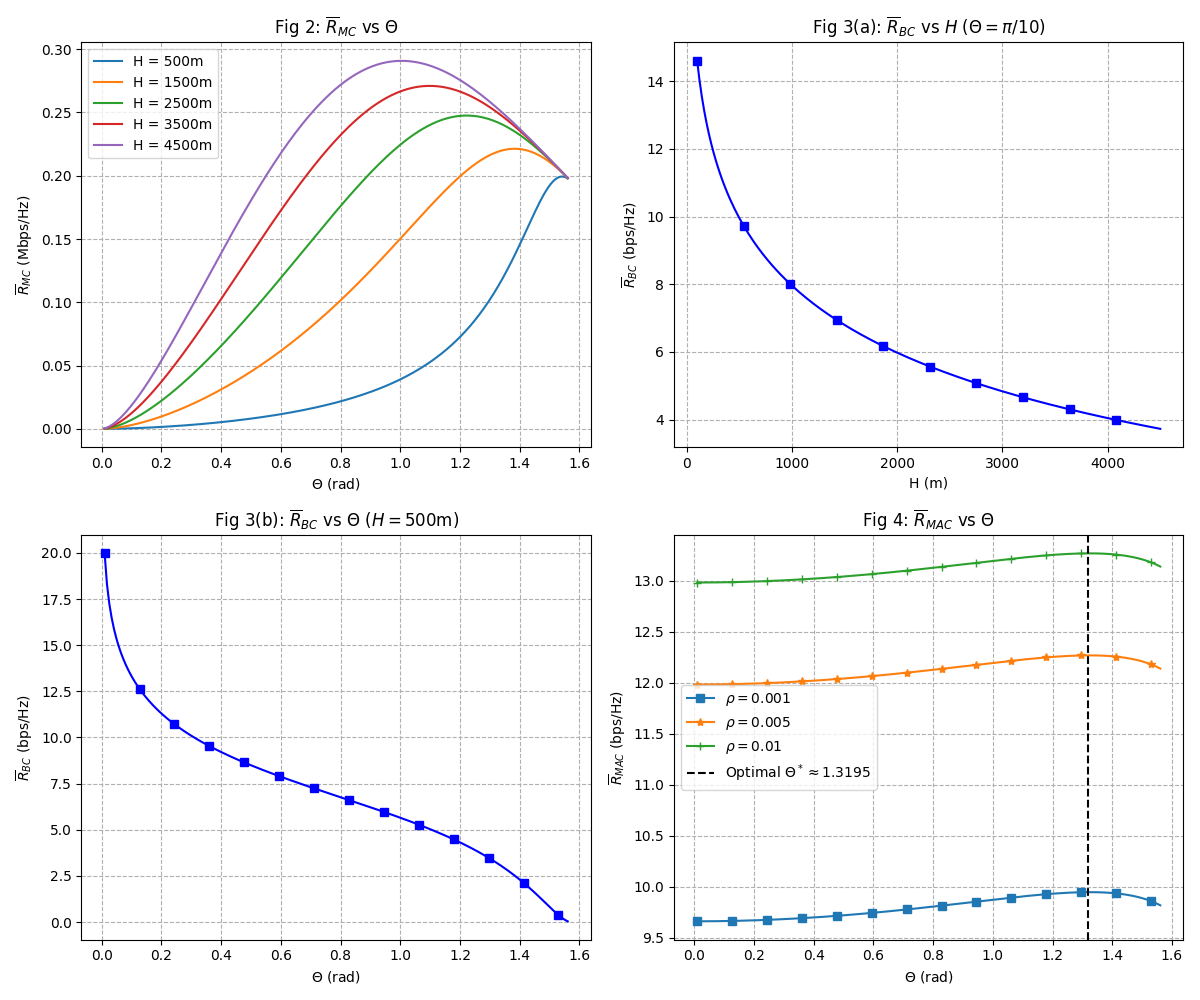
\includegraphics[width=0.95\textwidth]{Figure_1.png} 
    \caption{Reproduction of paper results: Multicast rate vs. $\Theta$ (top-left), Broadcast rate vs. $H$ and $\Theta$ (top-right, bottom-left), and Uplink MAC rate vs. $\Theta$ (bottom-right).}
    \label{fig:q4_reproduction}
\end{figure}

\section{Network Dimensioning and UAV Fleet Sizing}
To address the practical deployment of UAV networks, we evaluate the minimum number of UAVs required to satisfy a specific target rate per user,
$R_{target}$. We select the \textbf{Uplink Multiple Access (MAC)} model for this analysis.

Let the total geographical area be $A = 1,000,000 \text{ m}^2$ ($1 \text{ km}^2$), with a baseline ground terminal density
of $\rho = 0.005 \text{ GTs/m}^2$. The total number of users in the area is $K_{total} = \rho A$.
The total required system capacity to guarantee $R_{target}$ for all users simultaneously is $C_{req} = K_{total} R_{target}$.

As established in Section 3, the uplink MAC sum rate is independent of altitude $H$ and achieves a global maximum at an
optimal beamwidth of $\Theta^* \approx 1.3195 \text{ rad}$[cite: 9]. Consequently, a single UAV provides a strict capacity
ceiling of $\overline{R}_{MAC}(\Theta^*) \approx 13.2 \text{ bps/Hz}$. Therefore, the minimum number of coordinated UAVs
required, $N_{min}$, is given by the ceiling function:

\begin{align*}
N_{min} = \left\lceil \frac{K_{total} R_{target}}{\overline{R}_{MAC}(\Theta^*)} \right\rceil = \left\lceil \frac{\rho A R_{target}}{\overline{R}_{MAC}(\Theta^*)} \right\rceil
\end{align*}

Figure \ref{fig:q5_sizing} illustrates $N_{min}$ as a function of $R_{target}$ for both the baseline density ($\rho$) and a congested scenario where the user density increases by 20\% ($1.2\rho$). 

\begin{figure}[H]
    \centering
    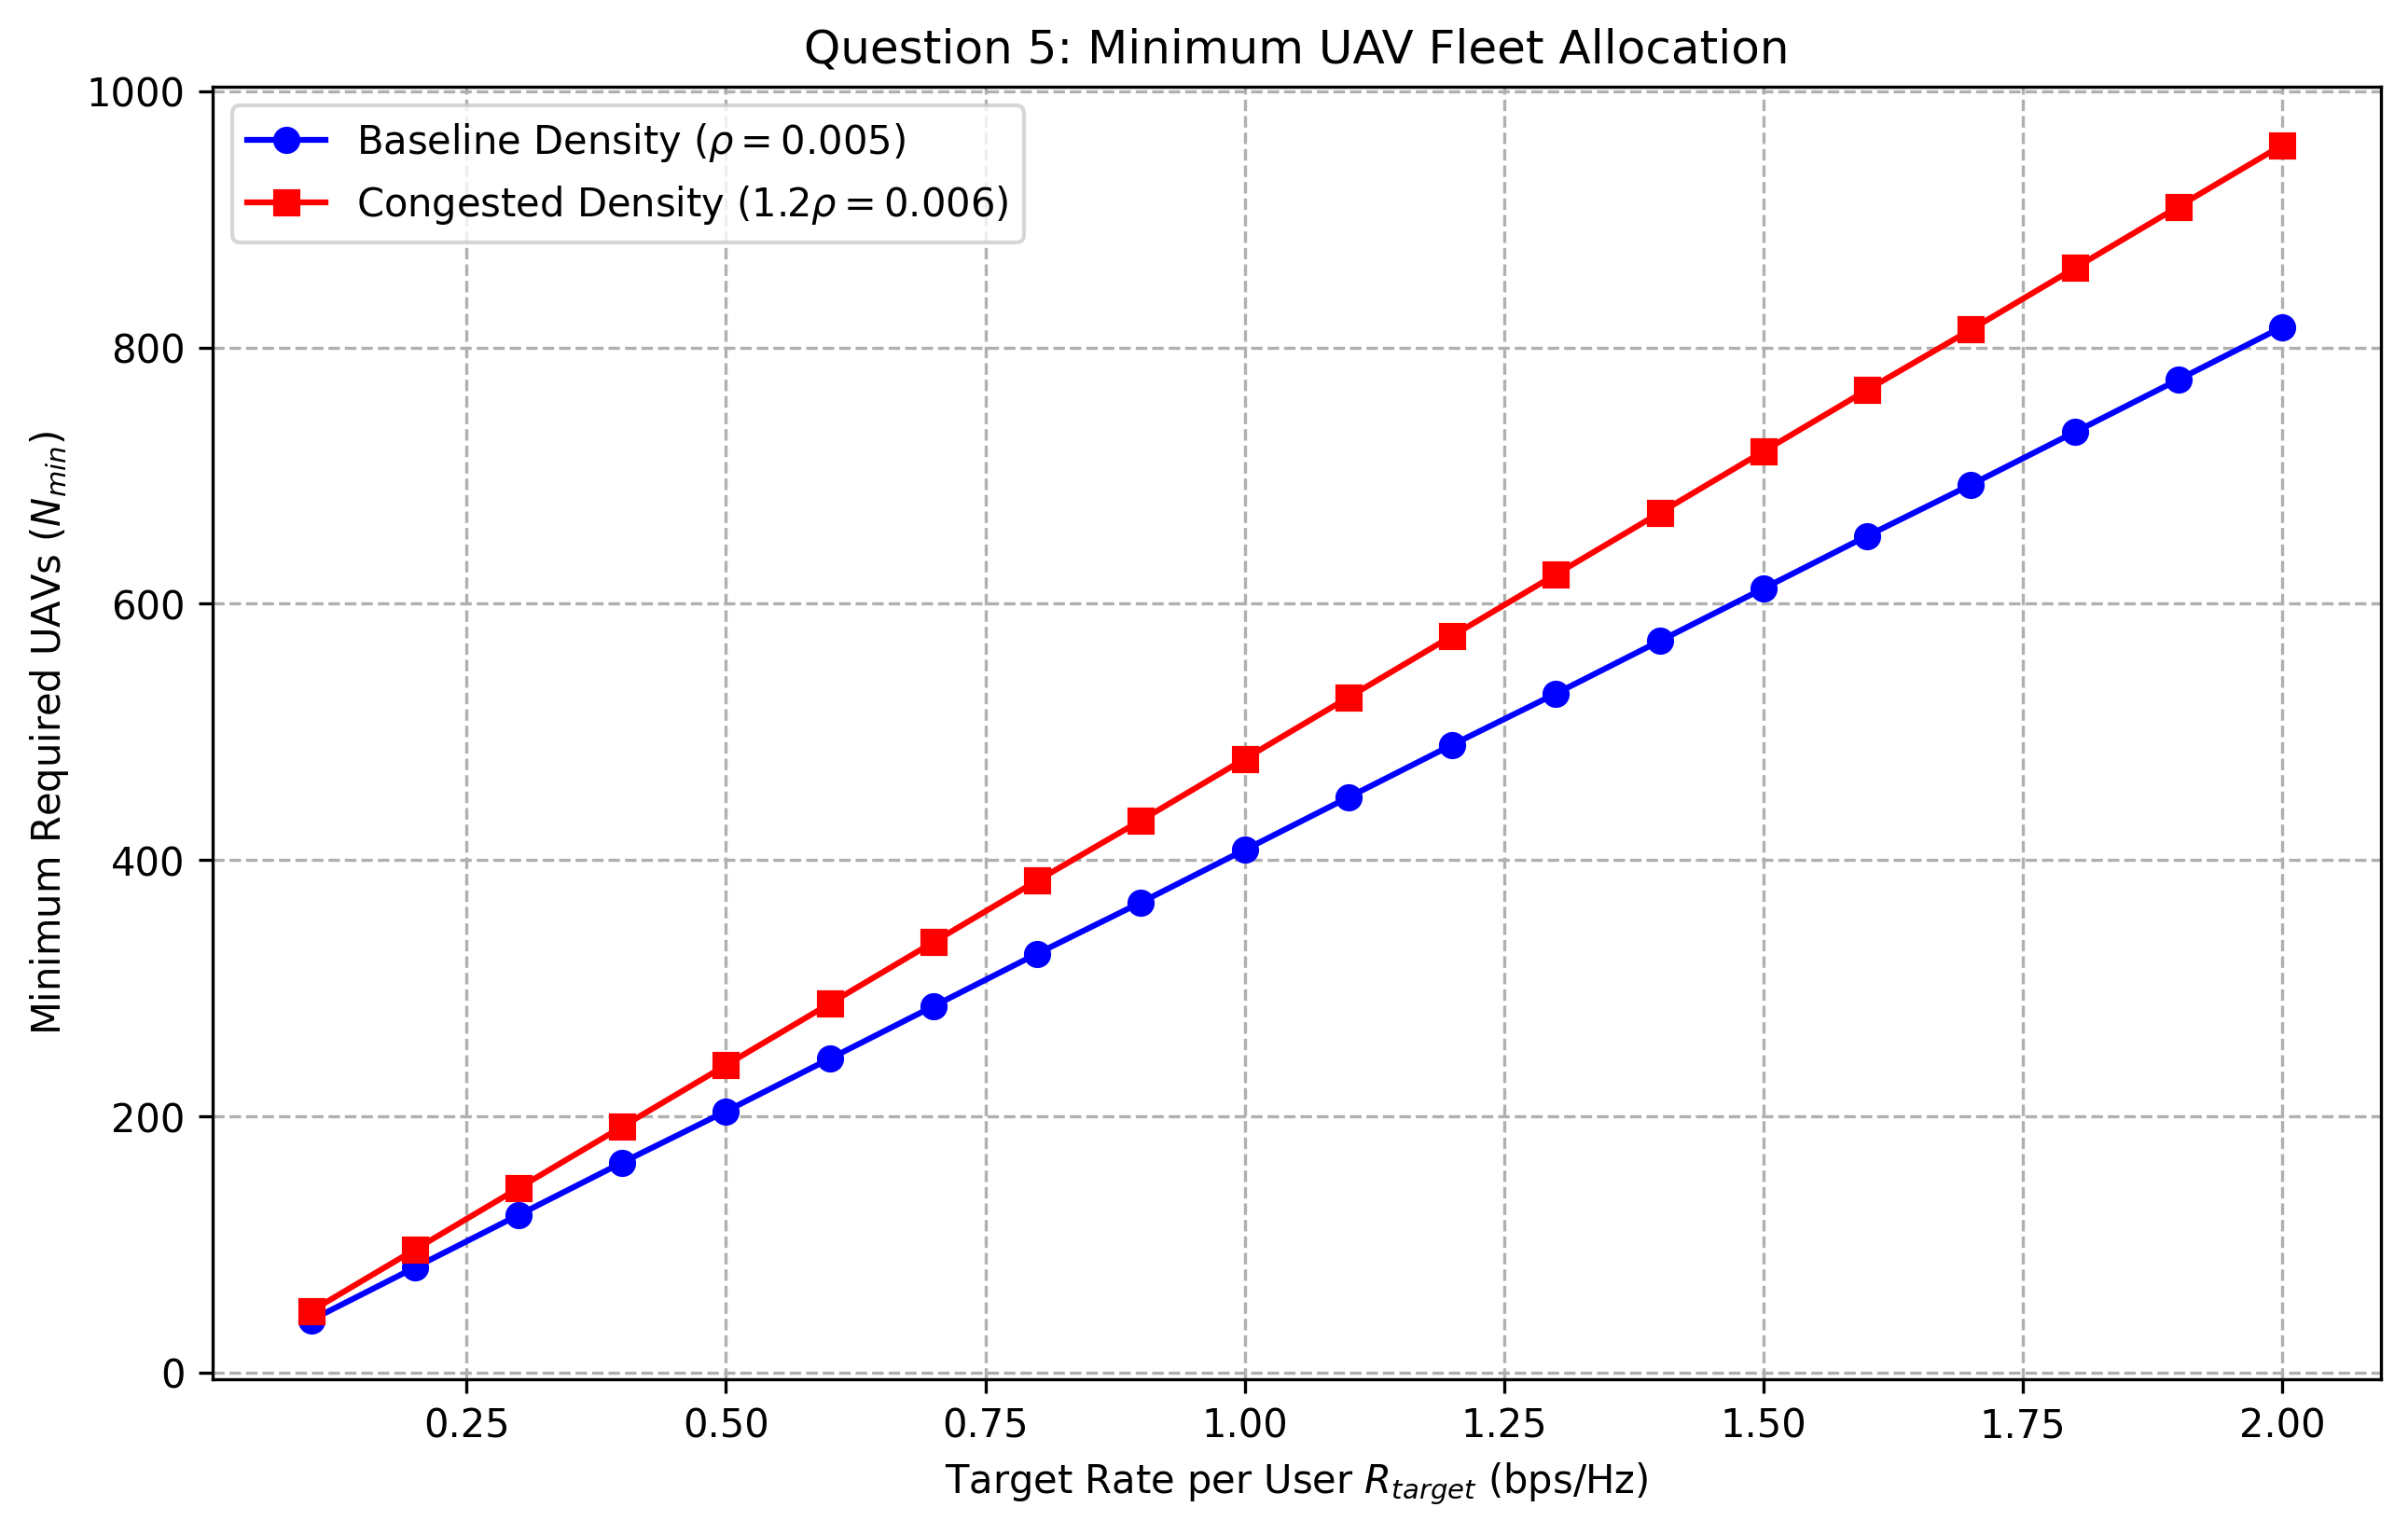
\includegraphics[width=0.8\textwidth]{q5_sizing.png} 
    \caption{Minimum required UAV fleet size vs. Target User Rate ($R_{target}$) for baseline and congested terminal densities.}
    \label{fig:q5_sizing}
\end{figure}

\subsection{Analysis of the Results}
The results demonstrate a strict linear scaling requirement. As the target rate per user increases,
the fixed capacity provided by a single UAV is rapidly exhausted, requiring the network operator to scale
out by deploying additional nodes to segment the geographical area into smaller, parallel service clusters. 

Furthermore, increasing the user density by 20\% uniformly shifts the fleet sizing requirements upward across
all target rates. This confirms that physical UAV deployment must scale proportionally with network
congestion. Because the maximum capacity per UAV is bounded by the physical channel and optimal beamwidth parameters,
the only variable left to accommodate a denser user base is an increase in the number of concurrent aerial platforms.

\newpage
\section{References}
    \begin{enumerate}
        \item H. He, S. Zhang, Y. Zeng and R. Zhang, “Joint Altitude and Beamwidth Optimization for UAV-Enabled ultiuser Communications,” in IEEE Communications Letters, vol. 22, no. 2, pp. 344-347, Feb. 2018, doi: 10.1109/LCOMM.2017.2772254.
        \item Course material from UAV13: Advanced Topics in Wireless Communications, Aristotle University of Thessaloniki (AUTh), 2026
    \end{enumerate}

\end{document}